\section{Real-world experiments}
TODO

\subsection{Setup}
TODO

\begin{figure}[!ht]
    \centering
    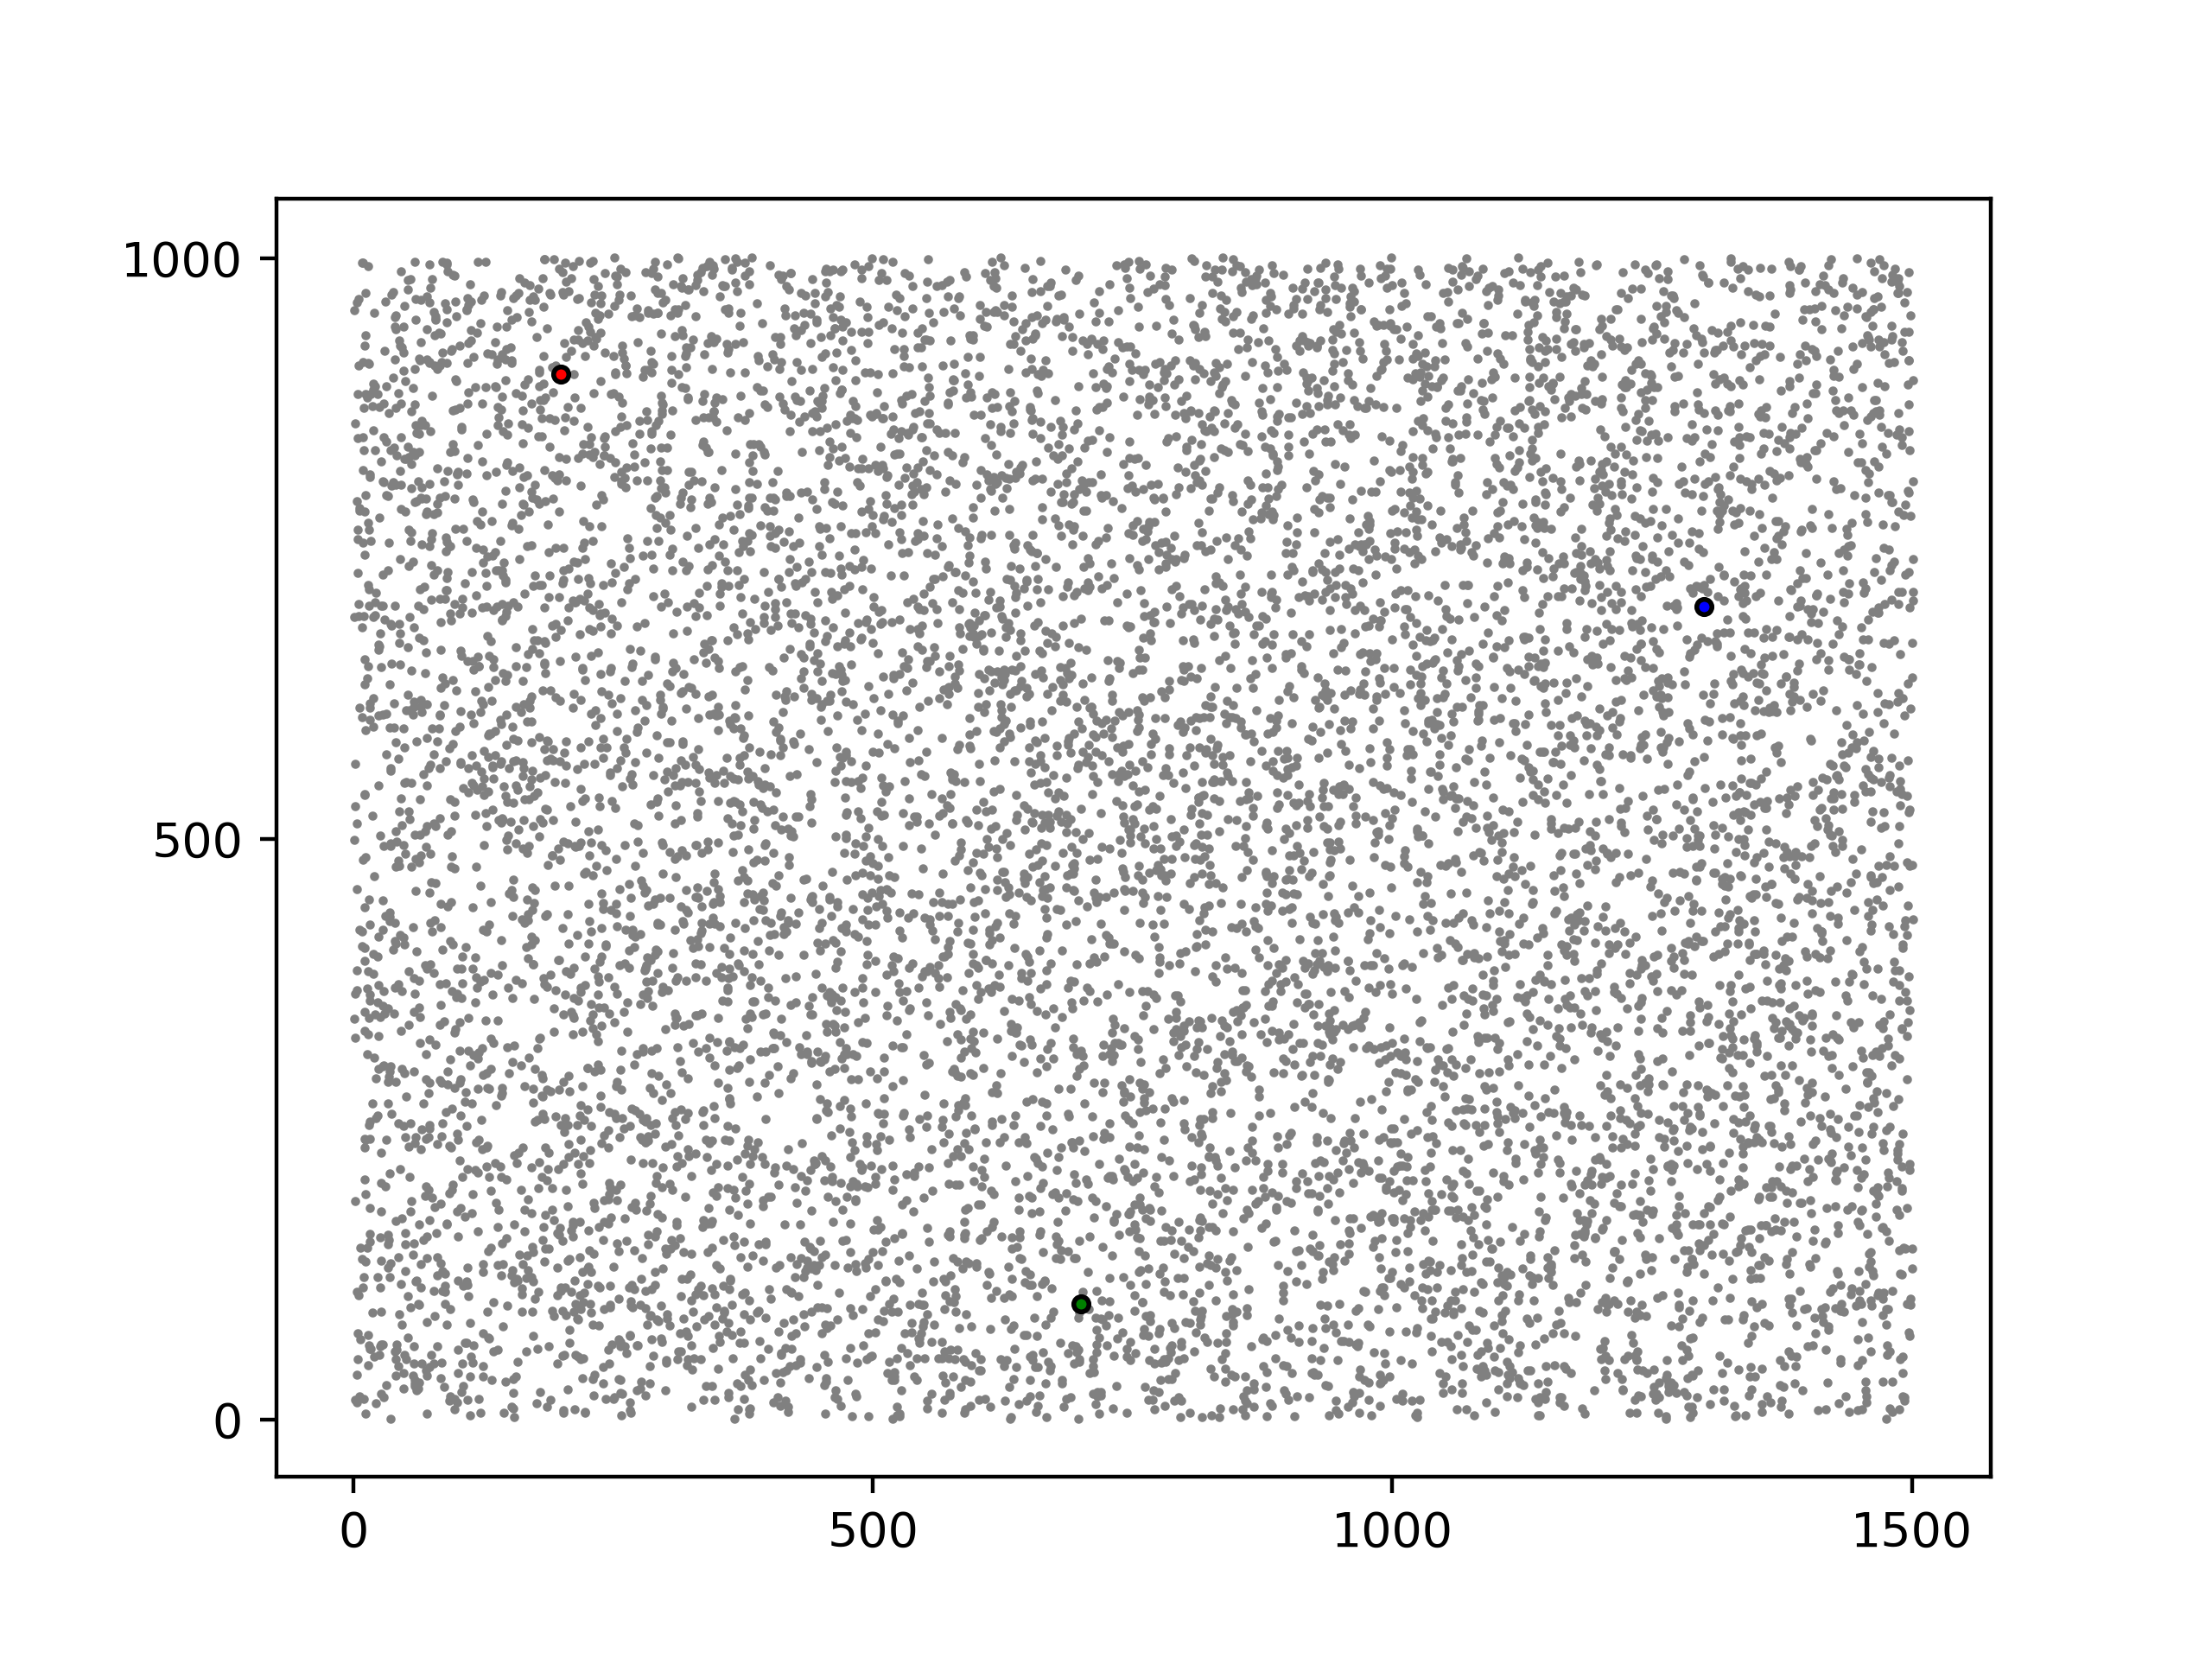
\includegraphics[width=\linewidth]{document/chapters/chapter_7/images/computation_start.png}
    \caption{Computation - Starting point}
    \label{fig:computation_start}
\end{figure}

\begin{figure}[!ht]
    \centering
    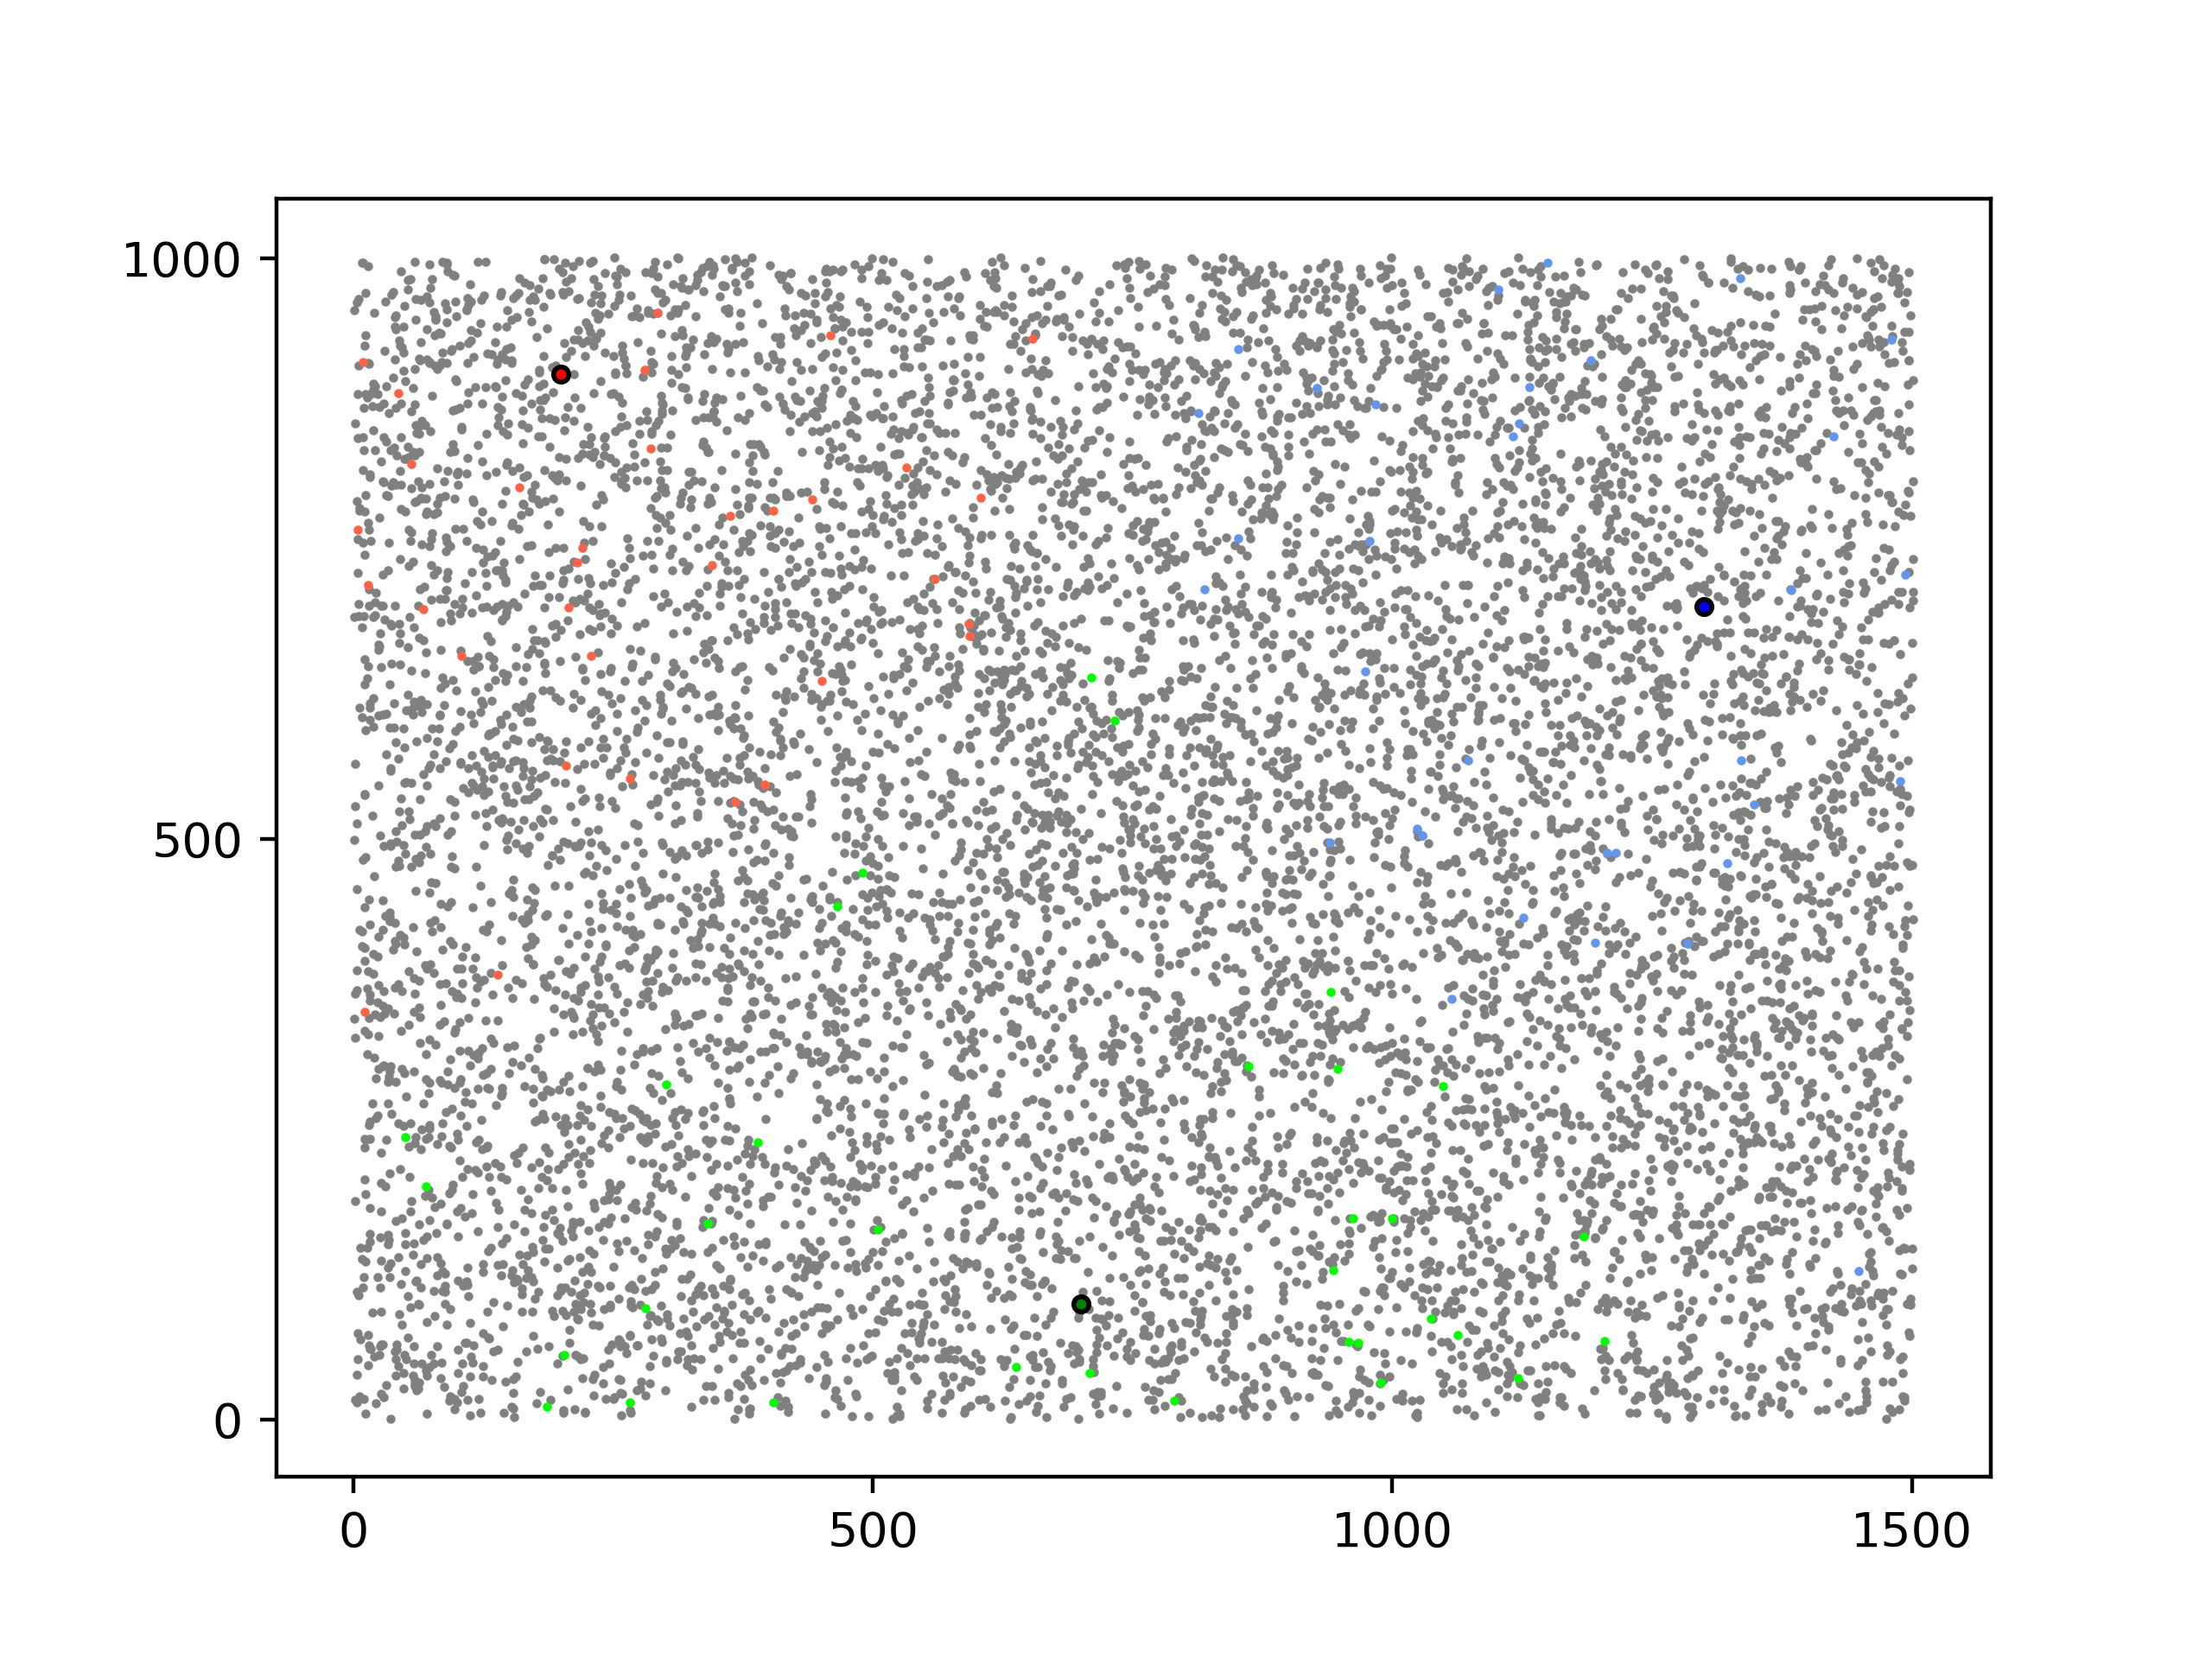
\includegraphics[width=\linewidth]{document/chapters/chapter_7/images/computation_region_computation.png}
    \caption{Computation - Region computation}
    \label{fig:computation_region_computation}
\end{figure}

\begin{figure}[!ht]
    \centering
    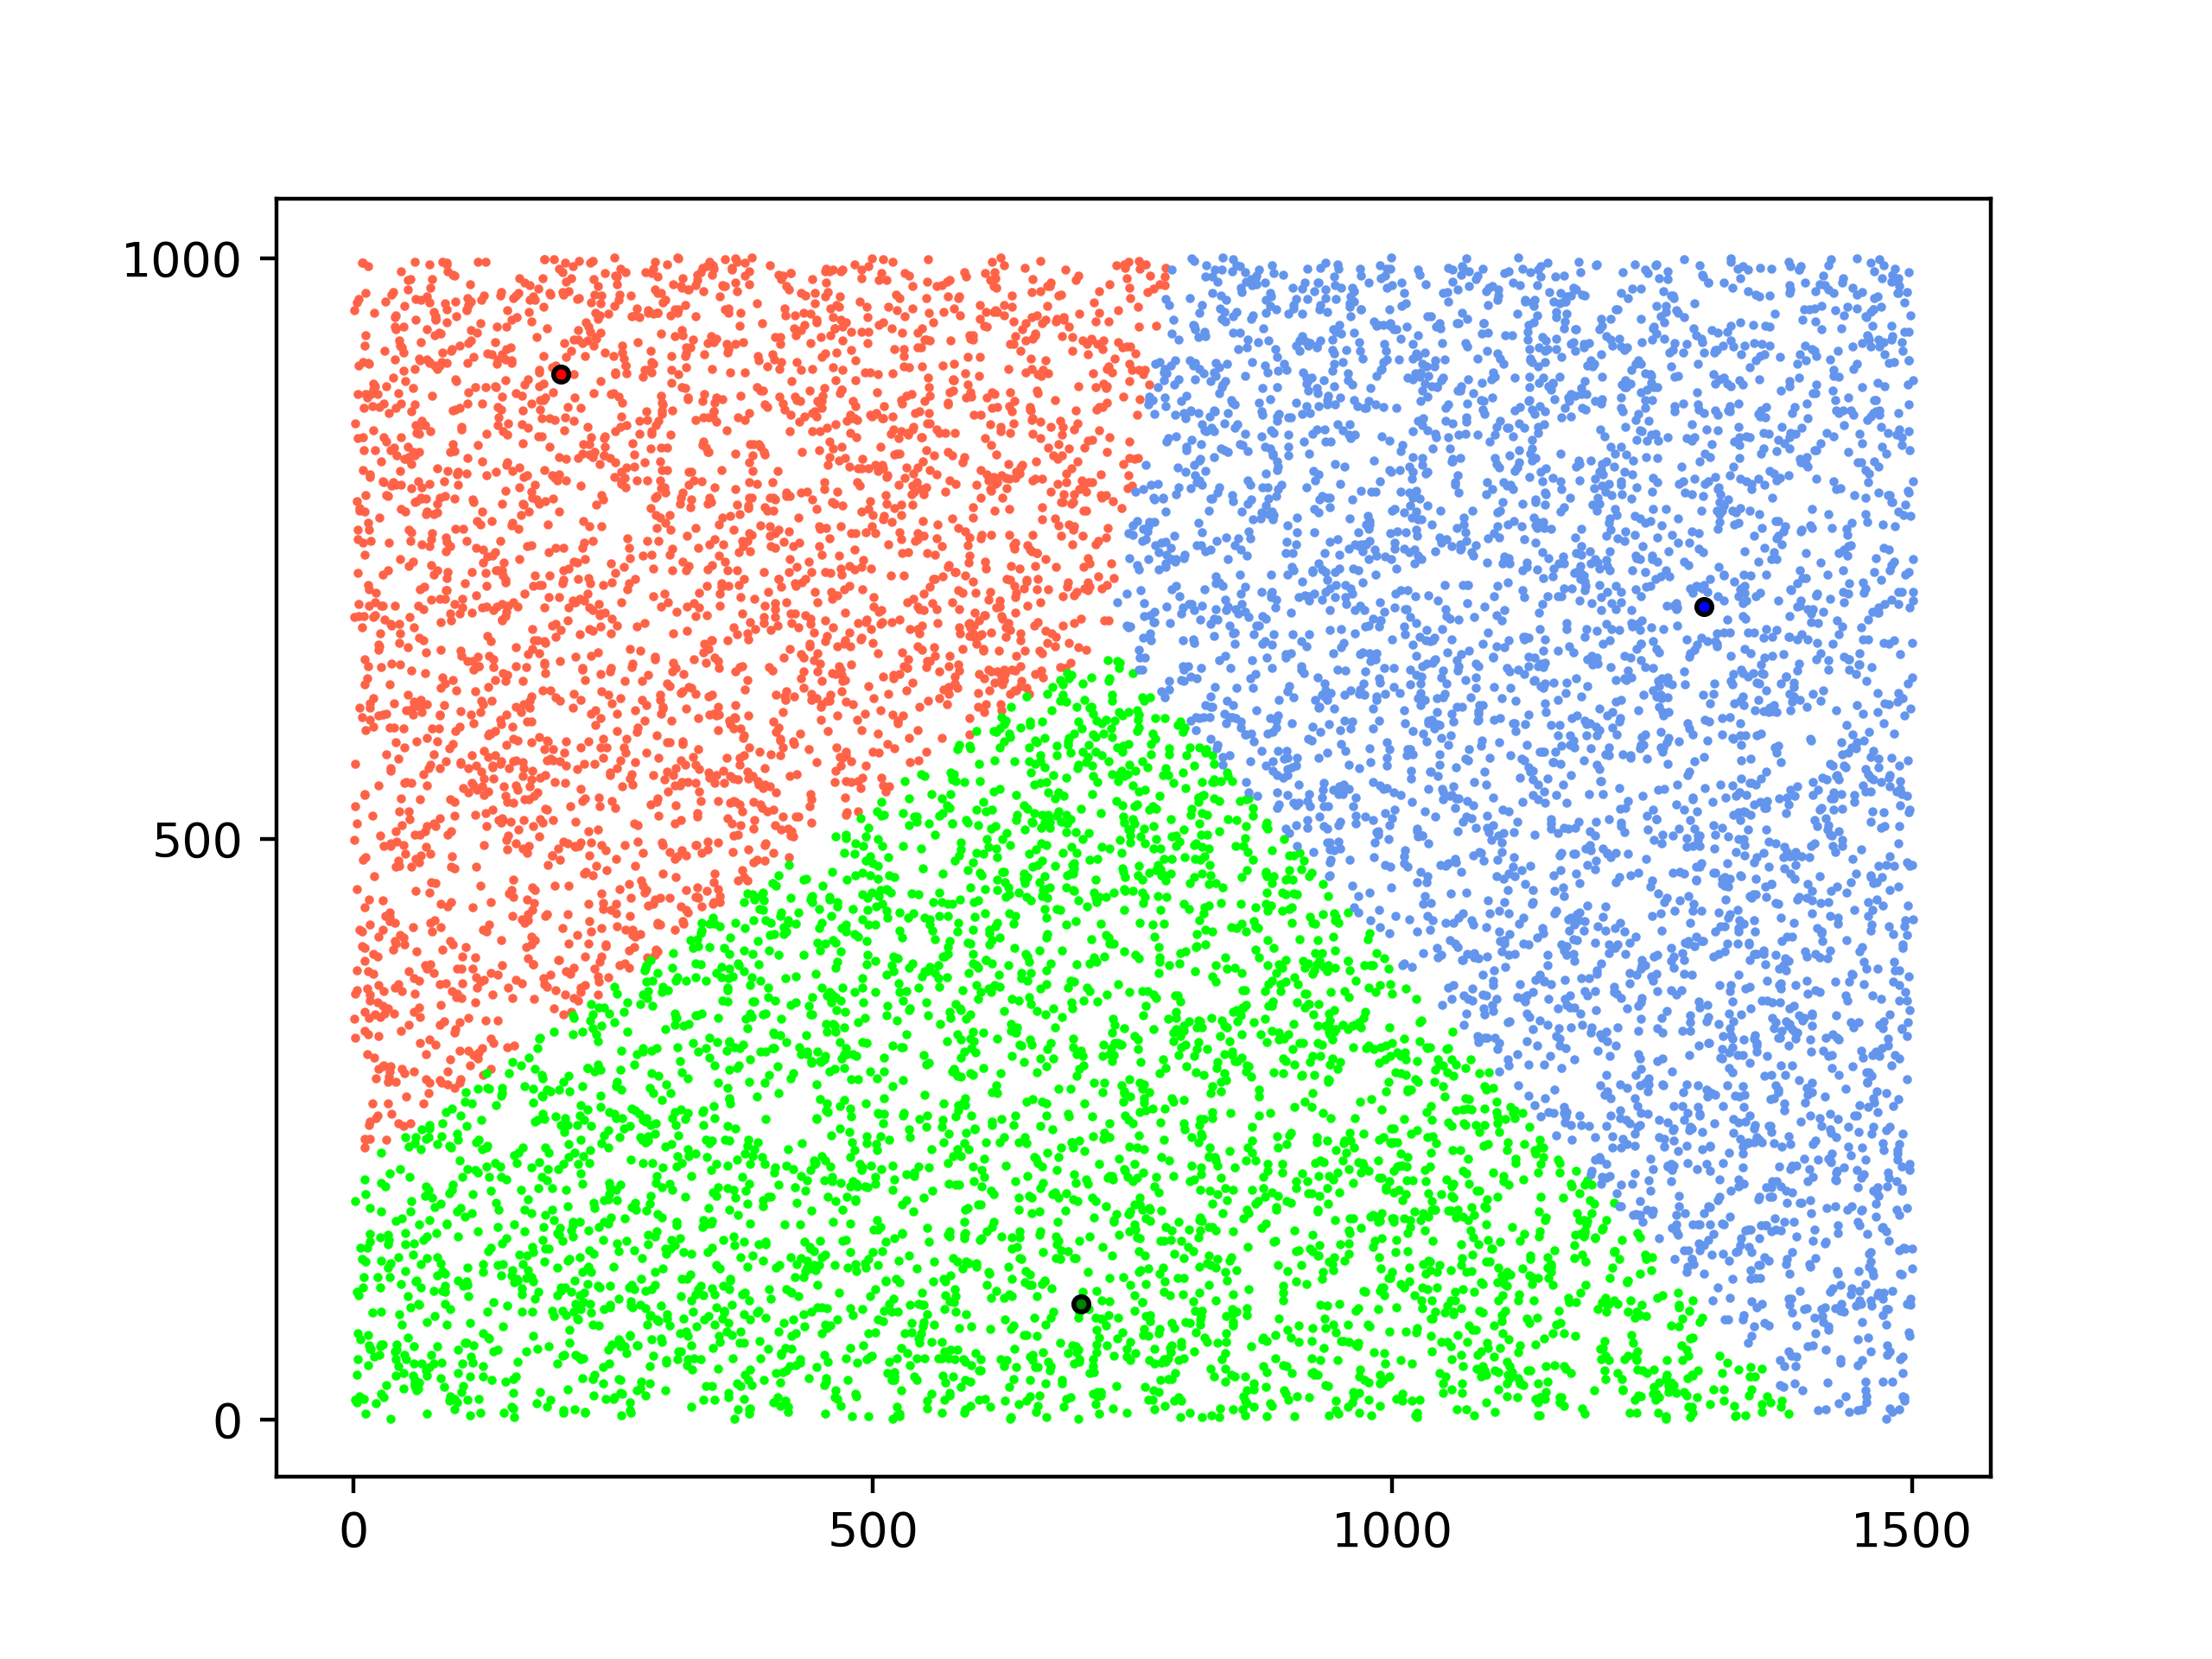
\includegraphics[width=\linewidth]{document/chapters/chapter_7/images/computation_final_result.png}
    \caption{Computation - Final result}
    \label{fig:computation_final_result}
\end{figure}

\subsection{Results}
TODO

\begin{figure}[!ht]
    \centering
    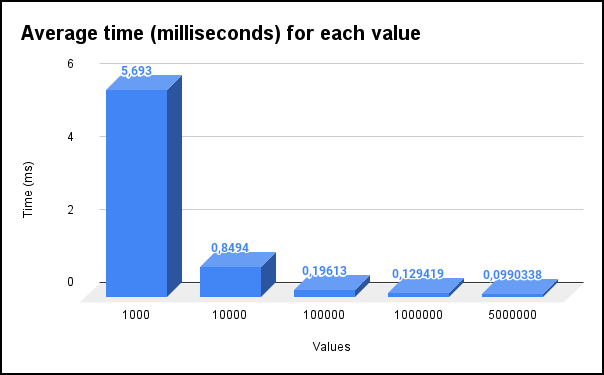
\includegraphics[scale=0.55]{document/chapters/chapter_7/images/experiment_results_avg_ms_per_value.png}
    \caption{Experiment results -}
    \label{fig:experiment_results_avg_ms_per_value}
\end{figure}